% intro.tex:

\chapter{Introduction}

\section{AI and Edge Computing}
\label{chap:intro:ai_and_edge}

\ac{DNN}s currently represent the state of the art in complex regression and
classification problems in image recognition, sequence to sequnce learning
\cite{dnn_is_sota_seq2seq}, speech recognition \cite{dnn_is_sota_speech}. As
such they are being deployed on both cloud platforms and edge devices at scale.

\ac{CNN}s are a variant of \ac{DNN}s that demonstrate great accuracy in
image/video recognition. The main computation layer of \ac{CNN}s that consumes
most of the runtime of a network is the convolutional layer. A convolution layer
operates on multi-demension tensors as part of a \ac{CNN}s feature extraction
portion of the network. Convolution layers exhibit a
significant amount of parallel behavior and data reuse. Additionally, the tight
latency, throughout and energy constraints imposed on CNN's in various
enviornments, particularly on edge devices has led to the proliferation of
customized hardware accelerators for \ac{CNN}s with particular emphasis on
accelerating convolution layers. 


\section{Convolution accelerators}
\label{chap:intro:cnn_accelerator_design_approaches}

Prior work on \ac{CNN} accelerators design can broadly be
classified based on 1) their target execution platform \ac{ASIC}/\ac{FPGA} 2)
Their target for acceleration, either entire layers of the network or
specifically convolution layers and finally 3) Their mathematical interpretation
of the convolution operation as either fundementally a matrix operation post
reorganization of its input tensor or a conventional stencil based operation. In
the next section, the strengths and weaknesses of the afformentioned approaches
will be discussed.

\section{Problem Definition}
\label{chap:intro:prob_def}

Regardless of the target execution platform chosen for a novel \ac{CNN}
accelerator architecture there exists a need to create a general enough
architecture that can support a wide variety of networks and network layer
types. \ac{CNN} \ac{ACC} generality can be decomposed into 1) Convolution
generality, which can be defined as the range of support convolution layers and
2) Network generality, whcih can be defined as the types convolution network
layers supported 

\ac{FPGA}s inherently have an advantage w.r.t architecture generality given
their reconfigurable nature. \ac{FPGA}-centric approaches incorporate the
architecture of a target \ac{CNN} network into their architecture compilation
process \cite{caffeine}. This allows \ac{FPGA}-based architectures to tackle
network generality by adding layer-spcific accelerators (provided they are
available) at compile time, as well as tailor \ac{Conv} \ac{ACC} primitives to
the target network in order to provide the appropriate amount of \ac{Conv}
generality and performance. The disadvantage of \ac{FPGA} based architectures is
1) The need to recompile the architecture prior to deployment of a new \ac{CNN}
with possibly no support for a new \ac{CNN} without recompilation 2) Inferior performance and energy
efficiency compared to a hardened architecture. One could harden a design
produced by an \ac{FPGA}-based architecture compilation process. However, this
will produce a design optimized for only one network and may not be general
enough. To the best of this author's knoweldge, no \ac{FPGA}-based \ac{ACC}
compilation processes incorporate more than one \ac{CNN} network architectures
into their architecture optimization process. 

\ac{ASIC}-based architectures tackle network generality by introducing a wide
variety of hardened layer accelerator primitives on-chip \cite{tpu}.
Additionally, they tackle convolution generality by either 1) Reinterpreting
convolution layers as \ac{GEMM} operations or 2) Creating a general
enough \ac{Conv} \ac{ACC} capable of supporting a wide range of \ac{Conv} layer
dimensions directly \cite{eyerissv2}. Given the pace of development in \ac{DNN}s,
new layers like \cite{transformer_model}'s self attention layer can
arise and become integral to improving \ac{DNN} model performance
\cite{conv_and_transformers}. These new layers may not be fully compatabile with
the chosen accelerator primitives in the \ac{ASIC}-based design approach and as
a result may only be partially accelerated. Additionally, \ac{ASIC}-based
designs must balance their dediction of on-chip resources to convolution vs
other resource intensive layers (e.g \ac{FC} layers) which may cause convolution
performance to suffer. Approaches that reinterpret convolutions to increase
convolution generality like \ac{GEMM} tend to dramatically increase data volume
which may strain on-chip memory resources as well as decrease energy efficicency
\cite{caffeine}. Finally, supporting a wide range of convolutions can come at
the cost of reduced performance/ energy efficiency for the statistical common
case of convolutions layer dimensions in a wide range of \ac{CNN}s.  


\section{Solution Overview}
\label{chap:intro:solution_overview}

There exists a convolution accelerator architectural template that offers 1)
Improved performance/ energy efficiency for the common case of convolution
layers accross a broad range of \ac{CNN}s 2) Operational flexibility to be able
to compute a wide variety of convolution layers under various and possibly
uncommon configurations 3) The ability to partially or fully accelerate
computationly intensive layers that currently exist in the literature and ones
that may arise in the future 4) The configurability that enables the
architectural template to be modified based on available compute resources and a
target library of networks. To satisfy the afformentioned requirements, in this
thesis, the following is presented: 
\begin{enumerate}
    \item (ConvolutIon statIstics GAthere) \ac{CIGAR} a tool that enables \ac{HERO}'s data driven design
    \item A \ac{HERO} derived from a novel data driven design approach
    \item TEMPO a tool that optimizes \ac{HERO} configurations based on a target \ac{DNN} library and available compute resources 
    \item \ac{SAM} a novel descriptor driven on-chip memory primitive capable of orchestrating
    energy efficient on chip data movements within \ac{HERO}
    \item A HERO network compiler that compiles arbitrary networks written in
    pytorch down to SAM descriptors for on-chip data orchestration
    \item A cycle accurate simulation platform driven by a SystemC simulation
    backend and a python evaluation frontend that can assess a HERO configuration's
performance and energy efficiency on arbitrary models written in Pytorch
    \item An analysis of a HERO configuration's performance and energy efficiency
    when running all 695 Networks present in the PyTorch Image Models (TIMM) library of
    networks \cite{timm}
\end{enumerate}


\section{Thesis Structure}
\label{chap:intro:thesis_structure}

This thesis's structure is illustrated in \autoref{fig:intro}.
\autoref{chap:background:intro} discusses background and related work in the
literature. \autoref{chap:dda} introduces \ac{CIGAR} and the data aware design
approach from which \ac{HERO} is derived. \autoref{chap:arch_dimensioning}
introduces \ac{TEMPO} from which several candidate configurations of HERO are
found. \autoref{chap:data_orchestration} introduces the SAM primitive. 
\autoref{chap:net_compile} discusses HERO's network compilation process
and how SAM descriptor are generated from arbitrary models in Pytorch. Finally
\autoref{chap:hero:sim_platform} discusses the HERO simulation platform as well
as results from running a HERO configuration optimized by TEMPO on all 695
networks in the TIMM library. 

\begin{figure}[ht]
  \centering
  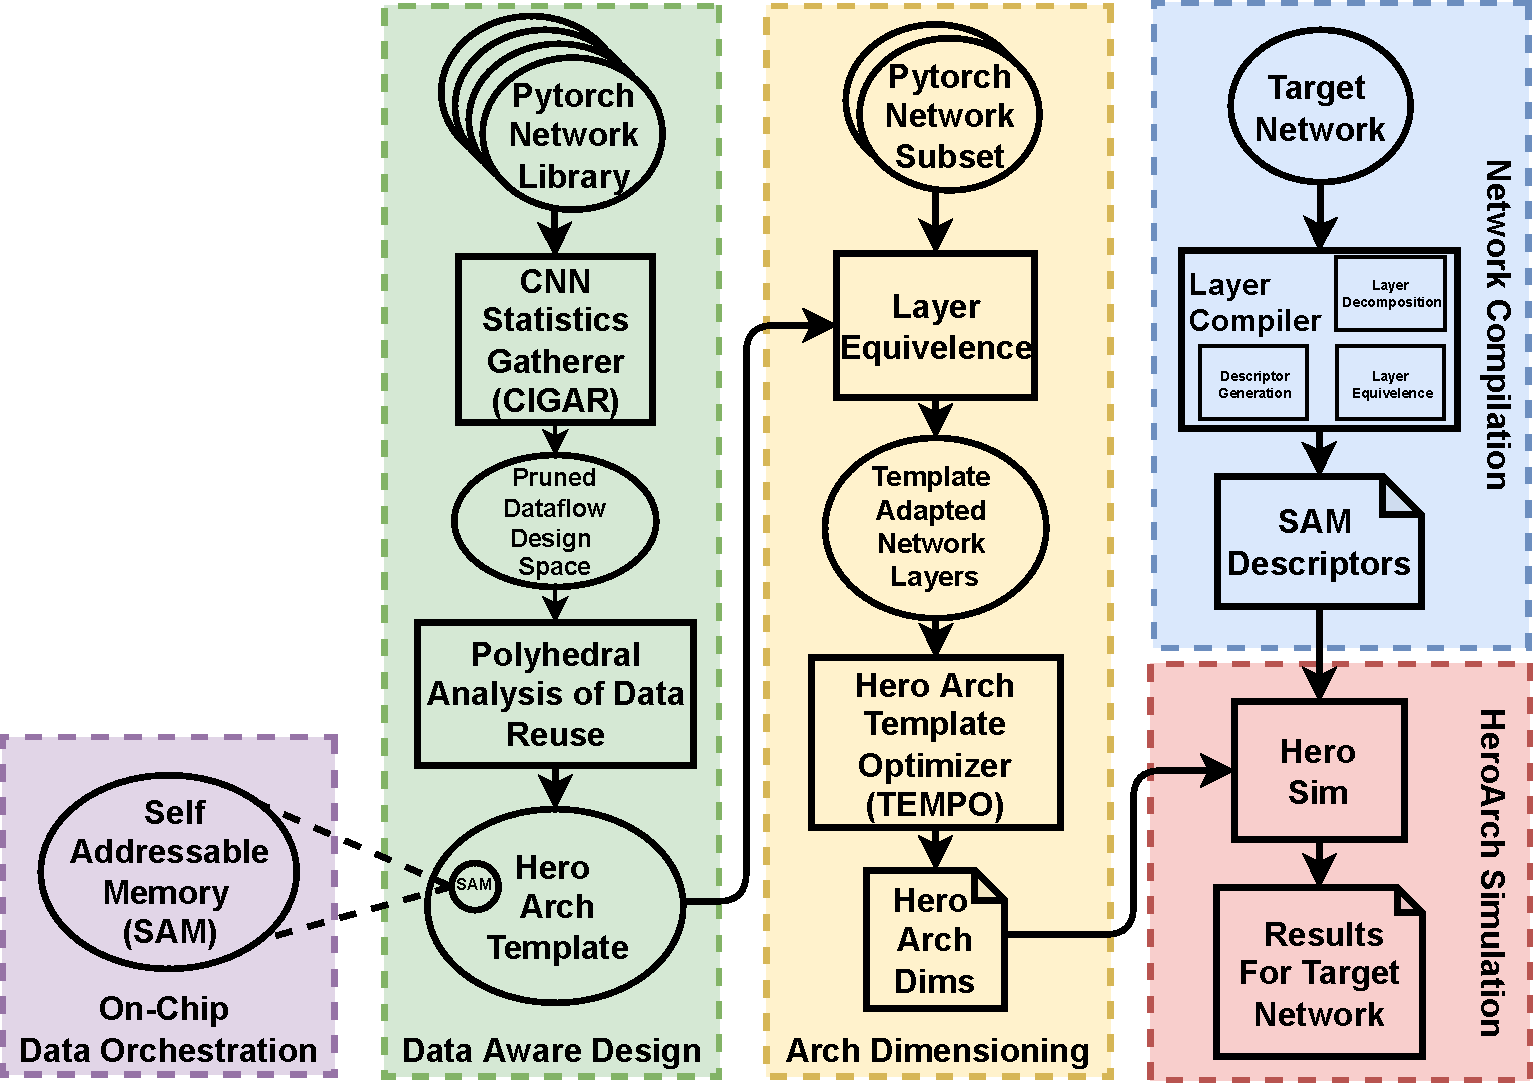
\includegraphics[scale=0.6]{fig/intro.pdf}
  \caption{Visual illustration of this thesis's content}
  \label{fig:intro}
\end{figure}